% 2011 年上海卷理科第 21 题：正四棱柱 ABCD-A1B1C1D1，O1 为 A1C1 与 B1D1 的交点。
% 来源 PDF：普通高考/2011/2011上海理.pdf（source id 见 manifest），第 2 页（印面 698）第 1 栏。
% 重绘依据：原图为斜二测式透视，A、D 在后侧上棱，B、C 在前侧上棱；A1、D1 在后侧下棱，
%   B1、C1 在前侧下棱。原图把交点标注为 O（题干写作 O1），本稿统一按题干标 $O_1$。
% 实线：可见棱 AB、AD、DC、BC，四条侧棱与底面可见边 B1C1、C1D1；
% 虚线：被遮挡的 A1B1、A1D1、A1A，以及题设用的对角线 AB1、AD1、A1C1、B1D1。
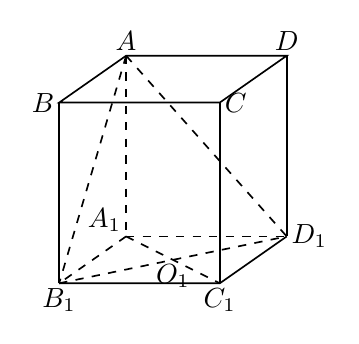
\begin{tikzpicture}[scale=0.85, semithick,
  every node/.style={inner sep=1.5pt}]
  % 上底面（后左 A、后右 D、前左 B、前右 C）
  \coordinate (A)  at (1.20,3.40);
  \coordinate (D)  at (3.60,3.40);
  \coordinate (B)  at (0.20,2.70);
  \coordinate (C)  at (2.60,2.70);
  % 下底面
  \coordinate (A1) at (1.20,0.70);
  \coordinate (D1) at (3.60,0.70);
  \coordinate (B1) at (0.20,0.00);
  \coordinate (C1) at (2.60,0.00);
  % 底面中心
  \coordinate (O1) at (1.90,0.35);
  % 可见棱
  \draw (A) -- (B) -- (C) -- (D) -- cycle;
  \draw (B) -- (B1);
  \draw (C) -- (C1);
  \draw (D) -- (D1);
  \draw (B1) -- (C1) -- (D1);
  % 被遮挡的棱
  \draw[dashed] (A) -- (A1);
  \draw[dashed] (A1) -- (B1);
  \draw[dashed] (A1) -- (D1);
  % 题设对角线
  \draw[dashed] (A) -- (B1);
  \draw[dashed] (A) -- (D1);
  \draw[dashed] (A1) -- (C1);
  \draw[dashed] (B1) -- (D1);
  % 顶点标注
  \node[above] at (A) {$A$};
  \node[above] at (D) {$D$};
  \node[left]  at (B) {$B$};
  \node[right] at (C) {$C$};
  \node[above left] at (A1) {$A_1$};
  \node[below] at (B1) {$B_1$};
  \node[below] at (C1) {$C_1$};
  \node[right] at (D1) {$D_1$};
  \node[below] at (O1) {$O_1$};
\end{tikzpicture}
